\chapter{Introduction}

In the last three decades a vast number of techniques for obstacle detection and evasion in mobile robots have been developed. While classical approaches include active range sensors, advancements in imaging hardware and processing power led to approaches which solely rely on visual information.

This chapter provides an overview of the particular obstacle detection problem that had to be solved, as well as an outline and evaluation of already existing approaches, finally leading to the actual method presented in this thesis.

\section{Motivation}

\begin{figure}[t]
 \begin{center}
  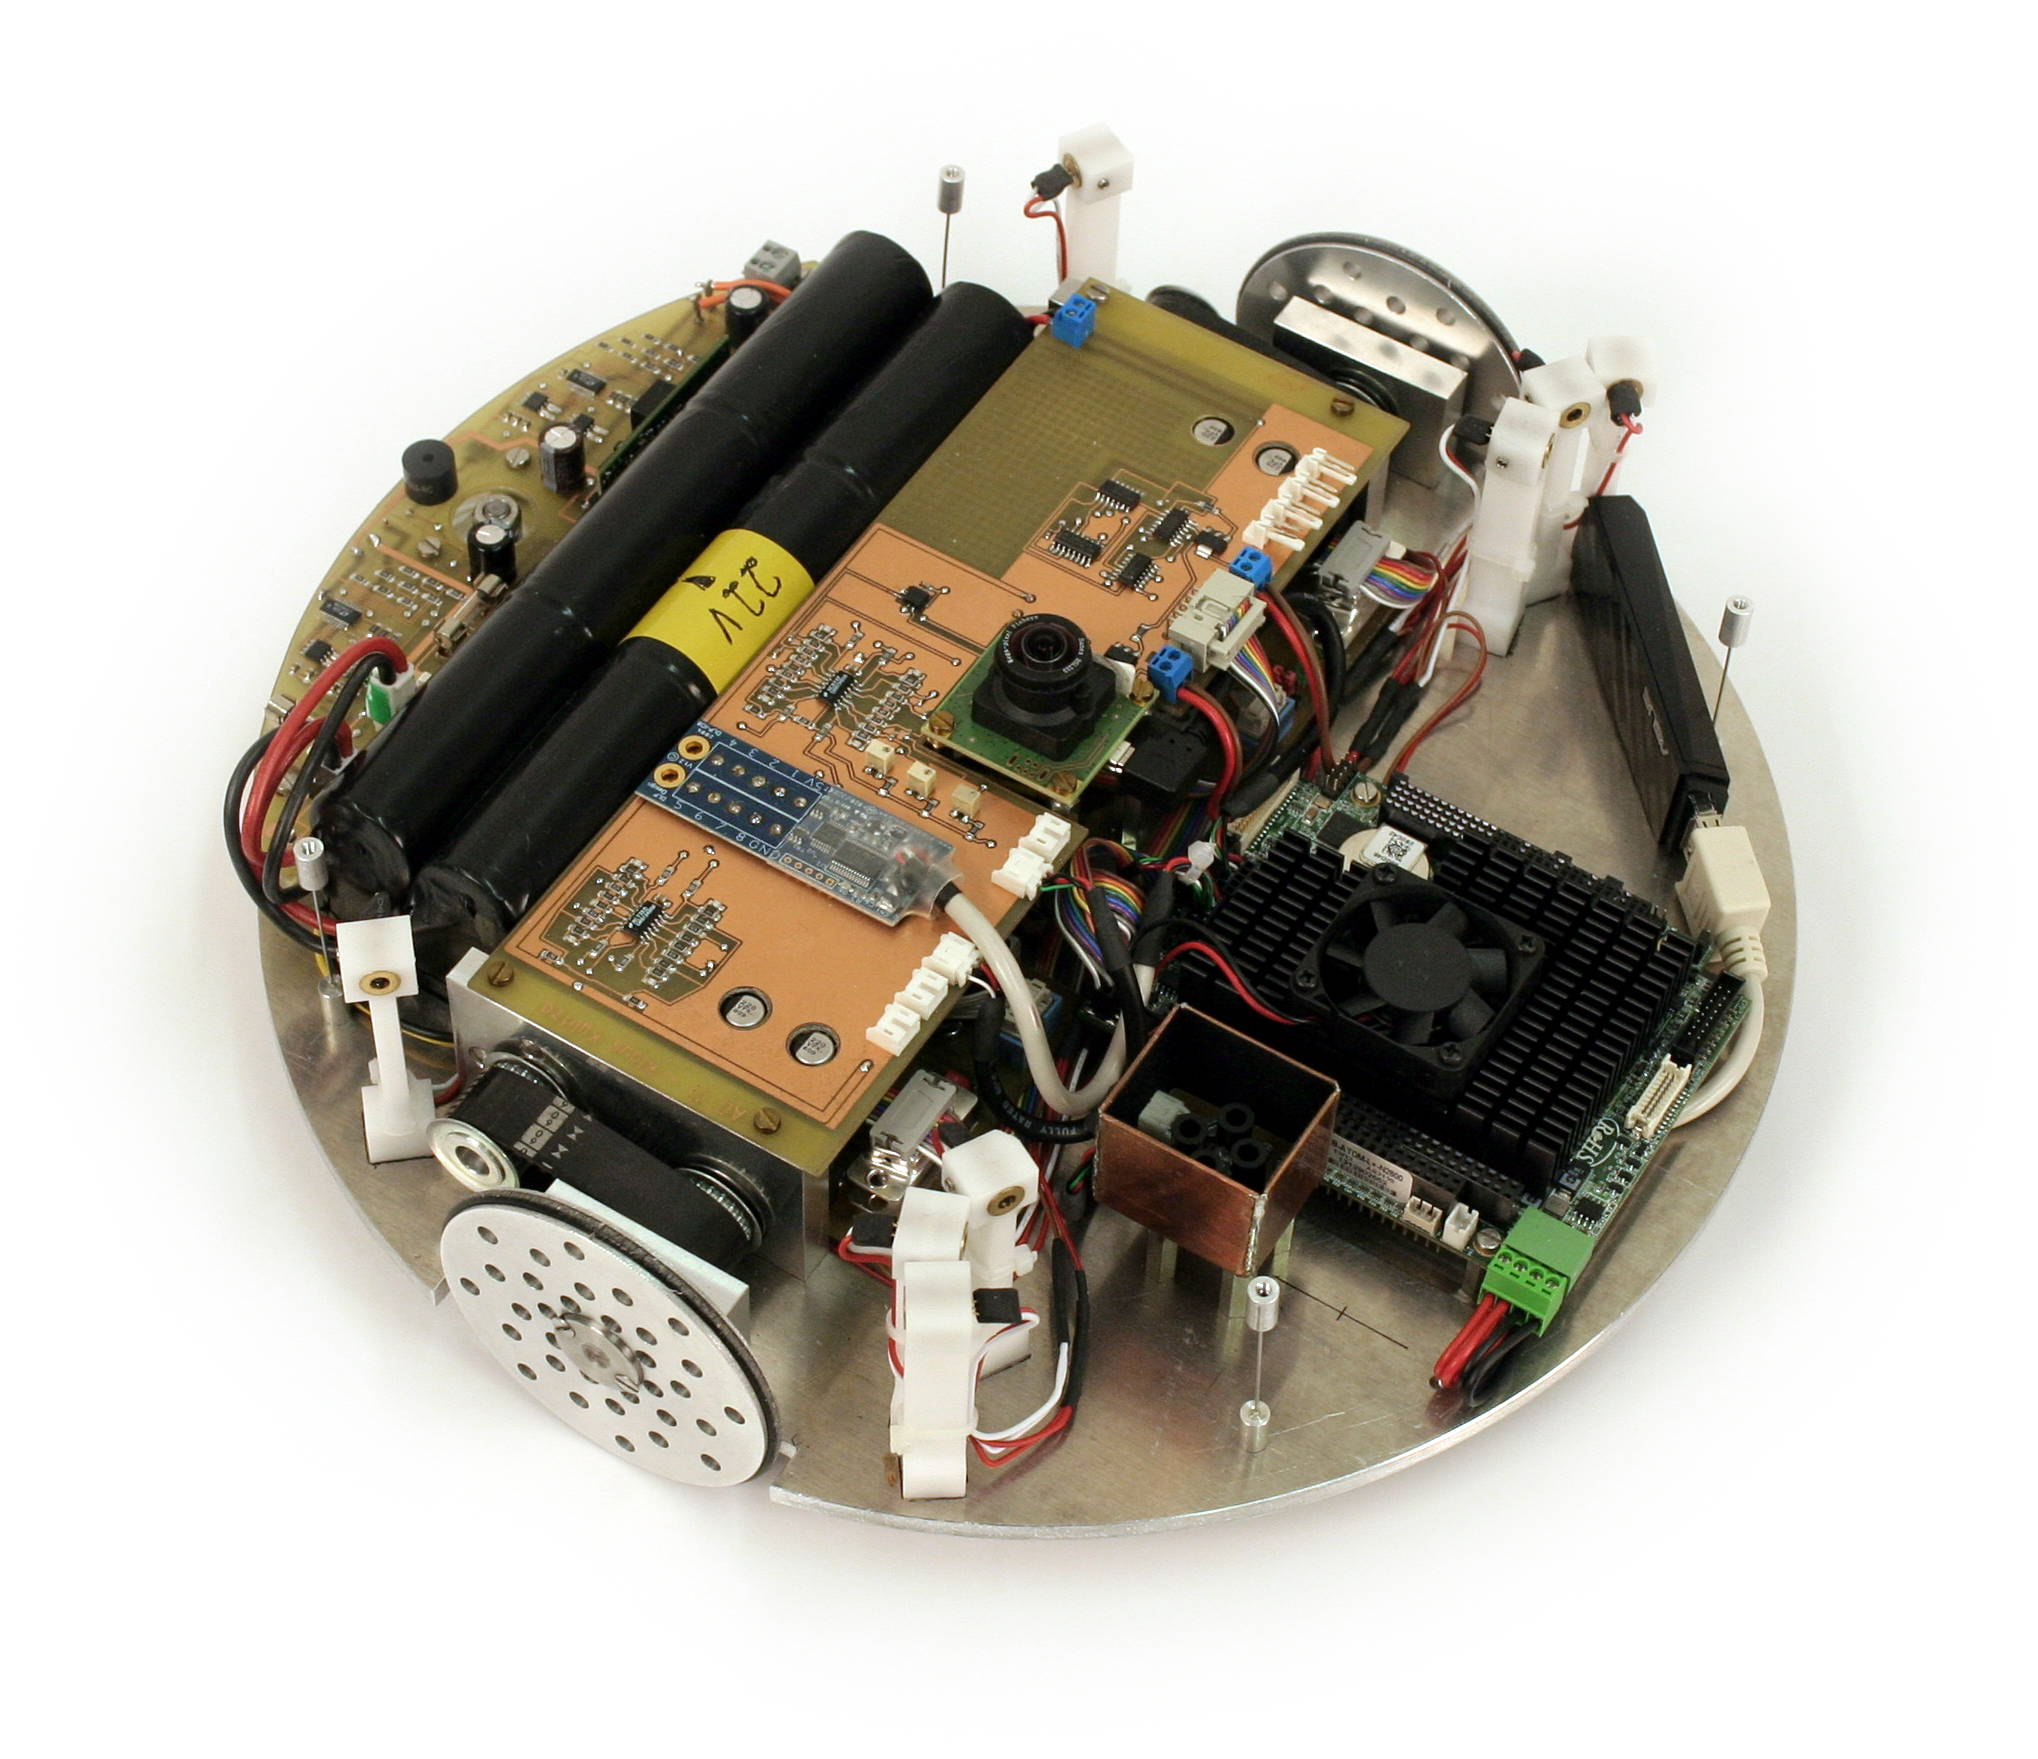
\includegraphics[width=0.8\textwidth]{media/nr6.jpg}
 \end{center}
 \caption{Photo of the robot platform (in-house development) as used in the experiments. One can see the eight laser diodes (mounted at the white holders) used for the coarse obstacle detection as well as the fisheye camera in the center of the platform and the on-board computer at the right side of the image. The radius of the entire system (including the cover not shown) is about $35\;\mathrm{cm}$, the top of the camera lens is located about $10\;\mathrm{cm}$ above the ground.}
 \label{fig:nr5}
\end{figure}

Obstacle detection and avoidance are crucial to most autonomous mobile systems, both biological and robotic. While mandatory for systems moving at high velocities in order to avoid physical damage, long-range obstacle detection is still a necessity for efficient navigation and route planning in applications like consumer-grade cleaning robots.

The target robot platform --- an in-house development inspired by such cleaning robots (see figure \ref{fig:nr5}) --- carries a set of eight static lasers diodes which are used for obstacle detection. The detection is performed by triangulating the laser points as they appear in an omnidirectional camera image. The usage of only four diodes at a time in conjunction with slow temporal sampling results in a relatively coarse environmental coverage, which likely causes small and slim objects to be missed.

Classical approaches to obstacle detection on mobile robots include sonar sensors and laser scanners, while more recent developments include time-of-flight cameras and structured light sensors \citep[chapter 4.1.9 ``Active ranging'', p. 125ff.]{AutonomousMobileRobots}. While laser scanners in particular provide a high spatial resolution, these solutions are specialized hardware components which might not be suitable for budget-constrained consumer devices. However, commercially available cleaning robots that employ laser scanner based obstacle detection exist\footnote{According to the manufacturer, laser scanner based obstacle detection is employed in their \textit{Neato} robot vacuum cleaner series (see \url{http://www.neatorobotics.com/}). Yet the laser scanner used here might not measure time of flight, but may instead be based on triangulation.}. Furthermore space, payload and electrical power restrictions can often force the hardware to be as simple and small as possible.

The availability of low-cost imaging hardware (partially caused by the widespread adaption of cameras in day-to-day electronic devices) and the emergence of small, powerful microprocessors with low energy footprint allow for cost-effective integration of image processing systems into mobile robots. Therefore a monochrome, upward directed camera equipped with a fisheye lens, allowing omnidirectional vision, is already built into the robot platform and --- besides the coarse laser based obstacle detection --- utilized for navigation using min-warping \citep{own_moeller10_1,own_hillen_13_1}.

The goal of this thesis is to deduce an obstacle detection algorithm from a fundamental optical flow equation and finally to provide a real-time solution capable of exploiting the visual information provided by the visual sensor. Obstacle detection is thus turned from a hardware into a mere software problem.

\section{Special requirements}

\label{sec:intro_special}

In order to allow real-time operation of the entire robot, the obstacle detection algorithm must stay within a certain time budget. As the algorithm has to run along numerous other processes and a new image is captured approximately every $200\,\mathrm{ms}$, the execution time of the obstacle detection method should stay well below $50\,\mathrm{ms}$ on an embedded Intel\textregistered\ Atom\texttrademark\ N2600 dual core CPU running at $1{.}60 \, \mathrm{GHz}$.

Another requirement concerns the vertical range in which obstacles need to be detected: The robot only has a height of about $10\;\mathrm{cm}$, hence obstacles lying far above that height do not need to be detected. In fact, detecting such obstacles (at least without height information) would be counterproductive, as it might prevent the robot from driving beneath furniture.

The requirements are relaxed by the fact that the robot is aimed at domestic indoor use, which allows to assume a relatively static world and a mostly even ground.

\section{Existing solutions}

\label{sec:existing_solutions}

Vision based obstacle detection is an active research area. Binocular vision is an approach often used in applications for which reliable obstacle detection in non-static worlds or in conditions without ego-motion is mandatory (for example automotive applications as in \citealp{650851}).

Fewer solutions exist for omnidirectional, monocular vision. The underlying idea of these approaches is to exploit the parallax information present in subsequent images captured under motion: Near objects show a relatively large displacement and can thus be detected.

The following list contains a selection of approaches suitable for the present camera setup:
\begin{description}
 \item[Direct analysis of non-sparse optical flow:] In this approach, non-sparse optical flow is estimated from a time series of images. The flow field is then directly fed into the motor controller in order to avoid obstacles. This approach can be biologically motivated, as for example insect flight is believed to be controlled by optical flow \citep{Egelhaaf:2009}. Early experiments with optical flow and flying robots have shown that this direct form of motor control is indeed practical \citep{doi:10.1117/12.131575}.

 \item[Free space detection:] As above optical flow is estimated from a time series of images and compared to the expected movement of the ground surface. Instead of direct motor control, free space regions with no obstacles are detected by analyzing the difference between the expected and measured flow vector field \citep{yoshizaki:inria-00325322}.

 \item[Feature-based optical flow and obstacle detection:] A sparse flow field is created by matching corresponding image regions in a time series of input images. This matching may be performed using either sparse optical flow estimation techniques and/or feature detectors like SIFT \citep{Lowe04distinctiveimage}. Single high velocity flow vectors then correspond to near obstacles.

 This method is for example described in a paper by \citet{Low05obstacledetection}, where an one-dimensional polar obstacle map (comparable to those obtained from a laser scanner) is built from a ``flow vector length to distance'' estimate.

 \item[Obstacles from depth:] Given the presence of a depth map which is reconstructed from the input images, classical approaches for robot navigation \citep[][chapters 5 and 6]{AutonomousMobileRobots} can be employed.

 Methods for depth reconstruction in monocular vision include \textit{shape from texture} and \textit{shape from shading}. Here depth information is reconstructed from still images under assumptions about texture distortion or lighting \citep{buelthoff1991shape}. Moreover, machine learning approaches can be applied to depth recognition in still images \citep{depthStill}.

 Reconstructing depth from a series of images captured at slightly different positions is called \textit{structure from motion}. Here a correspondence between feature points from at least two images is established. Besides performing depth reconstruction, the camera motion is estimated \citep[see][chapter 4.2.6 ``Structure from motion'', p. 181ff.]{AutonomousMobileRobots}.

 An example for \textit{structure from motion} in omnidirectional images on mobile robots can be found in \citet{kawanishi2013parallel}, where parallel vertical lines are extracted as features in order to allow operation in textureless artificial environments.
\end{description}

\section{Algorithm overview}

In this section the approaches listed above are evaluated, followed by a brief summary of the solution presented in this thesis.

\subsection{Limitations of the approaches presented above}

The algorithm presented in this thesis follows the \textit{obstacles from depth} design scheme:

An insect-like, direct control scheme is not suitable for efficient, pre-planned trajectories. Free space detection as proposed by \citeauthor{yoshizaki:inria-00325322} cannot be used, as the omnidirectional camera on the robot platform does not cover the range below the image horizon and thus does not see the ground. In fact, it is noteworthy that many algorithms for obstacle detection in monocular, omnidirectional vision systems (including those mentioned above) are designed for a catadioptric camera system mounted on top of the robot, which allows to perceive the ground plane \citep{yasushi1999omnidirectional,kim2007omnidirectional}.

Feature-based approaches were also discarded, as preceding tests have shown that in usual domestic environments only few points of interest are present in the narrow ($\leq 10^\circ$) range above the image horizon, which is critical for obstacle detection.

Most \textit{structure from motion} methods also use feature points for depth reconstruction and as mentioned above try to estimate the camera motion between the images. Yet as the robot knows its current velocity from the odometry data, this motion information is not required. In addition these techniques --- including shape from shading and machine learning approaches --- may not be suitable for the real-time constraints given on an embedded system.


\subsection{General idea}

\begin{figure}[p]
 \begin{center}
  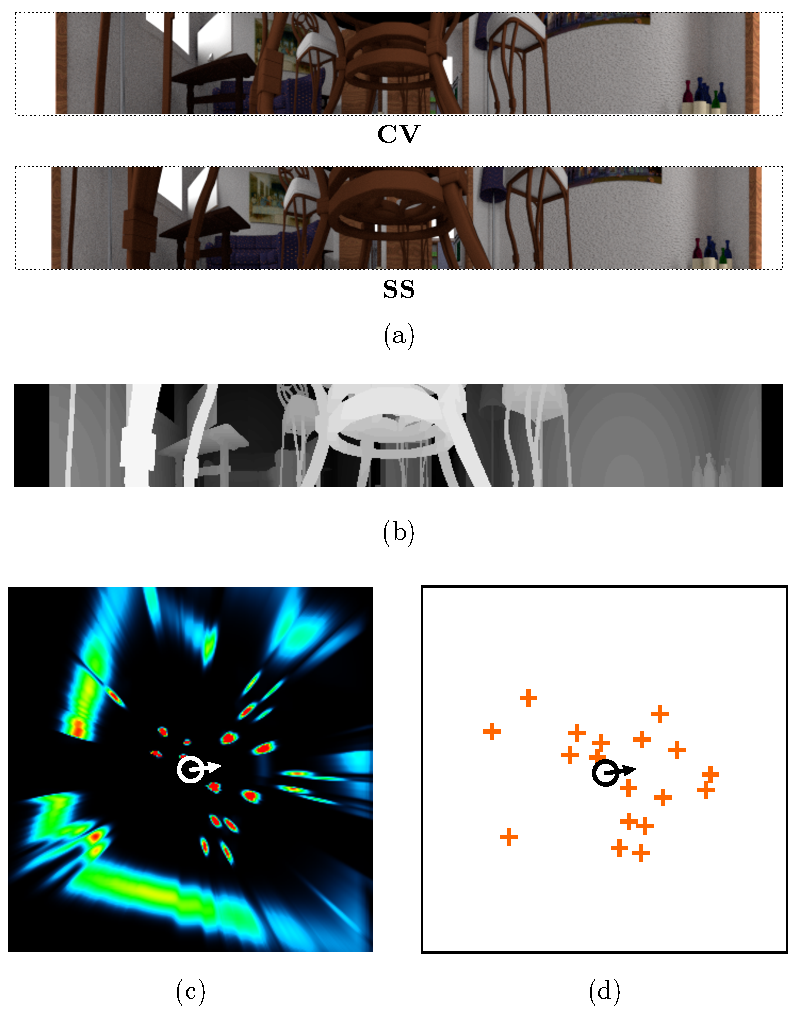
\includegraphics[width=0.8\textwidth]{media/general_idea2.pdf}
 \end{center}
 \caption{Conceptual overview of the stages in the obstacle detection algorithm:
 (a) A pair of panoramic input images (current view $\img{CV}$ and snapshot $\img{SS}$) is given (the actual images are monochrome). (b) Estimation of a depth map containing the distance for every pixel (image shows the ground truth). (c) The uncertainty distribution of each reconstructed pixel is accumulated in a top-down projected local environment map. (d) Clusters in the map with high density values are returned as obstacle points.}
 \label{fig:general_idea}
\end{figure}

Figure \ref{fig:general_idea} shows a short summary of the general idea of the algorithm: The depth reconstruction is performed by implicitly estimating optical flow. This flow estimation is accelerated by utilizing as much prior knowledge as applicable, including the motion information returned from the odometry sensors. Once the depth has been reconstructed, the resulting landmark points are projected onto a local top-down environment map in which the probability distributions accompanying each reconstructed surface point are accumulated. If a certain threshold is exceeded, the corresponding map region is emitted as an obstacle point.
